\section{Hypertext Transfer Protocol}
\label{section:http}

Το πρωτόκολλο επικοινωνίας HTTP (Hypertext Transfer Protocol) αποτελεί το πιο διαδεδομένο και ευρέως γνωστό
πρωτόκολλο στο χώρο του διαδικτύου. Αναπτύχθηκε από τους Tim Berners-Lee και την ομάδα του το 1990 και από τότε
έχει περάσει πολλές αλλαγές προκειμένου να μπορεί να ανταπεξέλθει στις ολοένα και συνεχώς αυξανόμενες ανάγκες του σήμερα.

Αποτελεί τη βάση κάθε μετάδοσης πληροφορίας στο διαδίκτυο. Στηρίζεται στην επικοινωνία δύο υπολογιστών, ενός που κάνει τα αιτήματα (client)
και ενός που απαντά σε αυτά (server). Στο τέλος της επικοινωνίας στην μεριά του παραλήπτη θα υπάρχει ανακατασκευασμένο
ένα ολοκληρωμένο αρχείο, από τα διάφορα υπο-αρχεία που μαζεύτηκαν, που μπορεί να είναι αρχεία ήχου, εικόνας, video.
Τα αιτήματα αυτού που ξεκινάει την επικοινωνία ονομάζονται requests, ενώ οι απαντήσεις του αποστολέα responses.

Η βασική δομή ενός http αιτήματος, η οποία φαίνεται και στο \autoref{fig:http_request}, περιληπτικά περιλαμβάνει τη μέθοδο (method) του αιτήματος, που περιγράφει
τη βασική λειτουργία του, το μονοπάτι (path) στο οποίο θα επικοινωνήσει με τον server, την έκδοση του πρωτοκόλλου που 
θα χρησιμοποιηθεί και τέλος headers προκειμένου να κρίνει ο server αν πρέπει να απαντήσει ή όχι πίσω στον client

\begin{figure}[!ht]
	\centering
	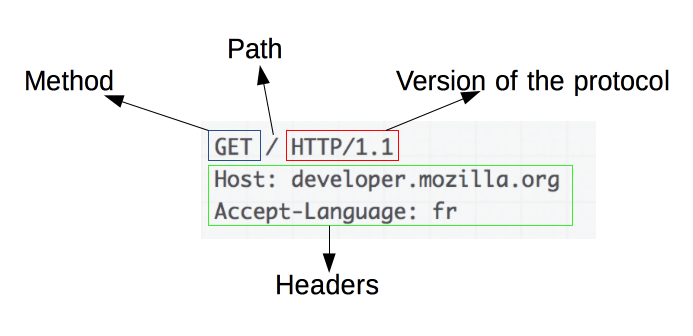
\includegraphics[width=0.7\textwidth]{./images/chapter2/http_request.png}
	\caption[Βασική Δομή ενός αιτήματος http]{Βασική Δομή ενός αιτήματος http}
	\label{fig:http_request}
\end{figure}

\subsection{Μέθοδοι}
\label{subsec:http_methods}

Πιο συγκεκριμένα οι βασικές μέθοδοι που παρέχει το http και οι συνήθεις λειτουργίες τους είναι οι εξής:

\begin{itemize}
	\item \textbf{GET}: παίρνει πληροφορία από τον server
	\item \textbf{POST}: υποβάλλει πληροφορία, προκαλώντας αλλαγές στον τρόπο λειτουργίας του server. Σχετίζεται συχνά με τη δημιουργία πληροφορίας που προηγουμένως δεν υπήρχε 
	\item \textbf{PUT}: όπως και πριν στέλνει πληροφορία στον παραλήπτη υπολογιστή, αλλά αυτή τη φορά επηρεάζει πόρους που ήδη υπήρχαν στο σύστημα. Σχετίζεται συχνά με την τροποποίηση ήδη υπάρχουσας πληροφορίας
	\item \textbf{DELETE}: διαγράφει από το σύστημα του server το συγκεκριμένο πόρο.
\end{itemize}

Αξίζει να σημειωθεί ότι πέρα από τις τέσσερις αυτές βασικές μεθόδους υπάρχουν και άλλες όπως είναι 
η \textbf{PATCH} που αποτελεί ειδική περίπτωση της PUT, η \textbf{HEAD} που αποτελεί ειδική περίπτωση της GET,
καθώς και άλλες που σχετίζονται με τη σύνδεση μεταξύ server και client. Αυτές είναι οι \textbf{CONNECT}, \textbf{OPTIONS} και \textbf{TRACE}.
Καθώς όμως, οι υπόλοιπες αυτές οι μέθοδοι, δεν χρησιμοποιούνται τόσο συχνά στην πράξη, δεν θα αναλυθούν περαιτέρω.

\subsection{Εκδόσεις HTTP}
\label{subsec:http_versions}

Η πρώτη έκδοση του HTTP, παρόλλο που δεν είχε κάποια συγκεκριμένo τίτλο, εκ των υστέρων ονομάστηκε 
HTTP/0.9. Αποτελεί την πιο απλή έκδοση του πρωτοκόλλου. Δεν υποστηρίζονταν headers και κωδικοί κατάστασης (status codes).
Εξυπηρετούσε μόνο GET αιτήματα και η μοναδική απάντηση που μπορούσε να επιστρέψει ήταν hypertext αρχεία. Kάθε φορά που ο server ανταποκρινόταν και έστελνε
απάντηση, η επικοινωνία με τον client έκλεινε κατευθείαν.

Στη συνέχεια και με την ανάπτυξη του διαδικτύου προστέθηκαν και άλλες λειτουργίες. Πέριξ του 1996,
με τη επόμενη έκδοση του πρωτοκόλλου (HTTP/1.0) τα αιτήματα πλέον συνοδεύονταν από headers, μεταπληροφορία σχετικά
με τη κατάσταση του αιτήματος, τον τύπο της πληροφορίας που περιμένουμε να έρθει (stylesheets, media, hypertext) καθώς και 
την έκδοση του HTTP που χρησιμοποιήθηκε στη συγκεκριμένη επικοινωνία. Επιπλέον πέρα από τη GET μέθοδο υπάρχει η
δυνατότητα για POST και PUT, δημιουργία και τροποποίηση πληροφορίας δηλαδή.

Στη συνέχεια το HTTP/1.1 προσπαθεί να βελτιώσει τις ήδη υπαρχουσες δυνατότητες κάνοντας την επικοινωνία
μεταξύ server και client πιο αποδοτική. Αντί να κλείνει η επικοινωνία μετά από κάθε μήνυμα, η σύνδεση παραμένει
ανοιχτή γλιτώνοντας έτσι μία σταθερή καθυστέρηση που υπήρχε σε κάθε αίτημα

Φτάνοντας στο σήμερα, μιλάμε για το HTTP/2.0 \cite{http2}. Αξιοποιώντας το πρωτόκολλο Speedy (SPDY) που αναπτύχθηκε κάποια χρόνια πριν
την κυκλοφορία του, και κτίζοντας πάνω σε αυτό, κατάφερε να μειώσει τους χρόνους επικοινωνίας server-client.
Μερικοί από τους τρόπους που επιτυγχάνεται αυτό είναι η μετατροπή του http από text πρωτόκολλο, σε δυαδικό (binary protocoll), επιτρέποντας έτσι χρήση καλύτερων
και αποδοτικότερων τεχνικών επικοινωνίας. Επιπλέον συμπιέζει τους headers (header compression) καθώς αποτελούν πληροφορία που
επαναλαμβάνεται όταν τα αιτήματα στον server είναι συνεχή. Ο server ακόμα, αποκτά έναν μηχανισμό (server-push) που του
επιτρέπει να προωθεί πληροφορία στον client (στην cache του client συγκεκριμένα), που δεν έχει ζητήσει ακόμα, αλλά βάση αυτού
που αιτήται, μάλλον θα ζητήσει εντός της ιδίας συνεδρίας.

Τέλος, πρέπει να αναφερθούμε στην τελευταία, αν και όχι ακόμα ευρέως διαδεδομένη, έκδοση HTTP/3.0. H βασική διαφορά με τους
πρωκατόχους του είναι ότι αλλάζει το πρωτόκολλο επικοινωνίας που χρησιμοποιεί όλα αυτά τα χρόνια, από TCP (Transfer Communication Protocoll) σε
έναν συνδυασμό UDP (User Datagram Protocoll) και QUIC (Quick UDP Internet Connections), μίας νέας τεχνολογίας που λύνει το πρόβλημα και βελτιστοποιεί τόσο το πρόβλημα 
της ασφάλειας των επικοινωνιών (TLS handshakes), όσο και της απώλειας πληροφορίας που μπορεί να υπήρχε λόγω UDP, πρωτοκόλλου που είναι γνωστό
για την ταχύτερη απόδοσή του σε σχέση με το TCP, αλλά και το γεγονός ότι είναι πιο επιρρεπές σε σφάλματα. Η νέα αυτή έκδοση από τα αποτελέσματα 
της \cite{http3}, φαίνεται να έχει ήδη καλύτερους χρόνους σε σχέση με τις παλαιότερες εκδόσεις και ήδη το 28\% του διαδικτύου αξιοποιεί τις δυνατότητές του. 


\subsection{Κωδικοί Κατάστασης}
\label{subsec:http_status_codes}

Οι κωδικοί κατάστασεις (status codes) αποτελούν μέρος της απάντησης του server. Επιτρέπουν στον χρήστη να καταλάβει με μία ματιά αν το αίτημα που έχει κάνει έχει επιστρέψει σωστά, ή έχει γίνει κάποιο λάθος στη μεριά του server.
Υπάρχουν πέντε μεγαλύτερες κατηγορίες που στεγάζουν όλες τις υποπεριπτώσεις αυτών. Πιο συγκεκριμένα:

\begin{itemize}
	\item \textbf{Εύρος 100-199}: Υποδηλώνουν ενημερωτική απάντηση σχετικά με τη λειτουργία του server
	\item \textbf{Εύρος 200-299}: Επιτυχή αιτήματα. 
	\item \textbf{Εύρος 300-399}: Υποδηλώνουν την ανακατεύθυνση του μηνύματος του client. Συνήθως συνοδεύονται από το νέο url στο οποίο πρέπει να αποσταλλεί το αίτημα
	\item \textbf{Εύρος 400-499}: Ανεπιτυχές αίτημα, που οφείλεται στον client. Ένα σύνηθες παράδειγμα είναι η αίτηση πρόσβασης σε προστατευόμενους πόρους χωρίς κάποιου είδους αυθεντικοποίηση, ή χωρίς τα σωστά στοιχεία για αυθεντικοποίηση
	\item \textbf{Εύρος 500-599}: Ανεπιτυχές αίτημα, που οφείλεται στον server. 
\end{itemize}